%% ============================================================
%%  Trading Book PnL FIFO – Technical Reference
%% ============================================================
\documentclass[11pt, a4paper]{article}

\usepackage[T1]{fontenc}
\usepackage[utf8]{inputenc}
\usepackage{lmodern}
\usepackage[margin=2.2cm]{geometry}
\usepackage{amsmath, amssymb}
\usepackage{booktabs}
\usepackage{array}
\usepackage{xcolor}
\usepackage{float}
\usepackage{enumitem}
\usepackage{fancyhdr}
\usepackage{titlesec}
\usepackage{parskip}
\usepackage{mdframed}
\usepackage{tikz}
\usetikzlibrary{shapes.geometric, arrows.meta, positioning, fit, calc, backgrounds}
\usepackage{listings}
\usepackage{microtype}
\usepackage{hyperref}

%% -- colours
\definecolor{TR_DARK}{HTML}{1a2744}
\definecolor{TR_BLUE}{HTML}{2e6fad}
\definecolor{TR_GREEN}{HTML}{27ae60}
\definecolor{TR_RED}{HTML}{c0392b}
\definecolor{TR_ORANGE}{HTML}{e67e22}
\definecolor{TR_GRAY}{HTML}{f2f4f8}
\definecolor{CODE_BG}{HTML}{f8f9fa}

%% -- page style
\pagestyle{fancy}
\fancyhf{}
\fancyhead[L]{\color{TR_DARK}\small\textbf{risk\_pylibrary} \textbar\ Trading Book PnL FIFO}
\fancyhead[R]{\color{TR_BLUE}\small\today}
\fancyfoot[C]{\color{gray}\thepage}
\renewcommand{\headrulewidth}{0.4pt}

%% -- section style
\titleformat{\section}{\large\bfseries\color{TR_DARK}}{}{0em}{}%
  [\color{TR_BLUE}\rule{\linewidth}{1.5pt}]
\titleformat{\subsection}{\normalsize\bfseries\color{TR_BLUE}}{}{0em}{}
\titleformat{\subsubsection}{\normalsize\bfseries\color{TR_ORANGE}}{}{0em}{}

%% -- code style
\lstdefinestyle{pycode}{
  backgroundcolor=\color{CODE_BG},
  basicstyle=\ttfamily\footnotesize,
  breaklines=true,
  frame=single,
  rulecolor=\color{TR_BLUE!40},
  keywordstyle=\color{TR_BLUE}\bfseries,
  commentstyle=\color{gray}\itshape,
  stringstyle=\color{TR_GREEN},
  language=Python,
  showstringspaces=false,
  aboveskip=4pt, belowskip=4pt,
}

%% -- tikz node styles (all use align=center for \\ support)
\tikzset{
  proc/.style={
    rectangle, rounded corners=4pt,
    minimum width=3.6cm, minimum height=0.75cm,
    text centered, align=center,
    draw=TR_DARK, fill=TR_DARK!10, font=\small},
  data/.style={
    rectangle, rounded corners=2pt,
    minimum width=3.2cm, minimum height=0.65cm,
    text centered, align=center,
    draw=TR_BLUE, fill=TR_BLUE!10, font=\small\ttfamily},
  dbbox/.style={
    rectangle, rounded corners=2pt,
    minimum width=2.8cm, minimum height=0.75cm,
    text centered, align=center,
    draw=TR_ORANGE, fill=TR_ORANGE!12, font=\small},
  decide/.style={
    rectangle, rounded corners=8pt,
    minimum width=2.8cm, minimum height=0.75cm,
    text centered, align=center,
    draw=TR_RED, fill=TR_RED!10, font=\small},
  cloud/.style={
    rectangle, rounded corners=10pt,
    minimum width=3.0cm, minimum height=0.70cm,
    text centered, align=center,
    draw=TR_GREEN, fill=TR_GREEN!12, font=\small},
  arr/.style={-{Latex[length=2.2mm,width=1.6mm]}, thick, color=TR_DARK!70},
  lot/.style={
    rectangle, rounded corners=3pt,
    minimum width=1.8cm, minimum height=0.7cm,
    text centered, align=center,
    draw=TR_BLUE, fill=TR_BLUE!15, font=\scriptsize},
  sell/.style={
    rectangle, rounded corners=3pt,
    minimum width=1.8cm, minimum height=0.7cm,
    text centered, align=center,
    draw=TR_RED, fill=TR_RED!15, font=\scriptsize},
  shq/.style={
    rectangle, rounded corners=3pt,
    minimum width=1.8cm, minimum height=0.7cm,
    text centered, align=center,
    draw=TR_ORANGE, fill=TR_ORANGE!15, font=\scriptsize},
}

%% =============================================================
\begin{document}

%% ---- Title Page
\thispagestyle{empty}
{\color{TR_DARK}
\vspace*{3cm}
\noindent\rule{\linewidth}{3pt}\\[0.5em]
{\huge\bfseries\color{TR_DARK} Trading Book PnL FIFO}\\[0.3em]
{\Large\color{TR_BLUE} Technical Reference}\\[0.3em]
\noindent\rule{\linewidth}{1pt}\\[1.5em]
{\large
  \texttt{automation/task\_pnl\_trading\_book.py}\\[0.3em]
  \texttt{risk\_models/pnl\_fifo.py}
}\\[2.5em]
{\normalsize\color{gray}
  Pipeline: \texttt{main\_run\_pnl\_fifo}
  $\;\to\;$ \texttt{initiate\_pnl\_engine}
  $\;\to\;$ \texttt{pnl\_realised\_polars}\\[0.5em]
  \today \quad|\quad Author: F.\ Balloni — Risk Modelling
}
}
\newpage

%% ---- TOC
\tableofcontents
\newpage

%% =============================================================
\section{Overview}

The pipeline computes \textbf{realised and unrealised P\&L} for the
fractional-share trading book using a strict
\textbf{First-In, First-Out (FIFO)} matching methodology.
The computation runs \emph{incrementally}: it reads the latest cached
open-position snapshot from Snowflake, processes all new trades
up to yesterday, and uploads refreshed position and cache parquet
files to S3.

\medskip
\begin{mdframed}[backgroundcolor=TR_GRAY, linecolor=TR_BLUE,
                 linewidth=1pt, roundcorner=4pt]
\textbf{Accounts processed:}\\[6pt]
\begin{tabular}{lll}
  \toprule
  Account    & Data Source          & Trade Query \\
  \midrule
  9800001301 & \texttt{share\_booking} & \texttt{old} \\
  9800003301 & \texttt{share\_booking} & \texttt{old} \\
  9800001601 & \texttt{inquisitor}     & \texttt{new} \\
  9800003601 & \texttt{inquisitor}     & \texttt{new} \\
  \bottomrule
\end{tabular}
\end{mdframed}

%% =============================================================
\section{Top-Level Task: \texttt{main\_run\_pnl\_fifo}}

\subsection{Purpose}

\texttt{main\_run\_pnl\_fifo} is the entry point called by the
Airflow DAG.  It queries the Snowflake P\&L cache table for the
last processed date per account, then calls
\texttt{initiate\_pnl\_engine} for each account with the
appropriate incremental date window.

\subsection{Pipeline Flow}

\begin{figure}[H]
\centering
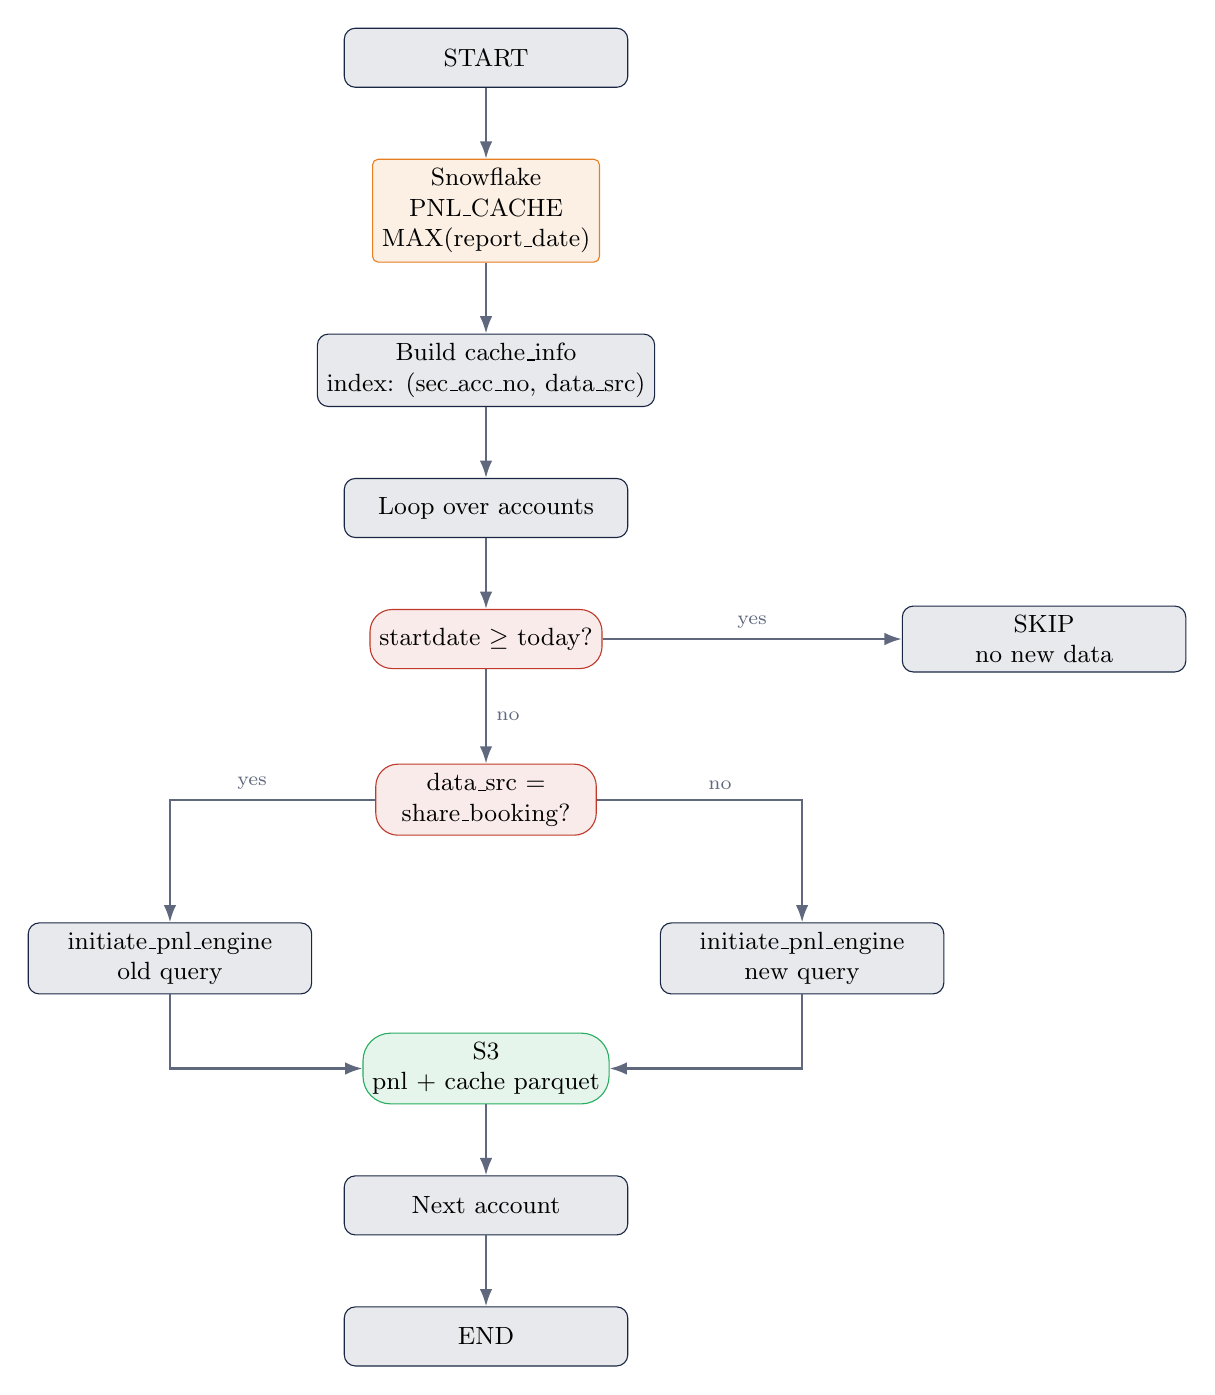
\begin{tikzpicture}[node distance=0.9cm and 0.5cm]

  \node[proc] (start)  {START};

  \node[dbbox, below=of start] (sf)
    {Snowflake\\PNL\_CACHE\\MAX(report\_date)};

  \node[proc, below=of sf] (ci)
    {Build cache\_info\\index: (sec\_acc\_no, data\_src)};

  \node[proc, below=of ci] (loop)
    {Loop over accounts};

  \node[decide, below=of loop] (skip)
    {startdate $\ge$ today?};

  \node[proc, right=3.8cm of skip] (skp)
    {SKIP\\no new data};

  \node[decide, below=1.2cm of skip] (src)
    {data\_src =\\share\_booking?};

  \node[proc, below left=1.1cm and 0.8cm of src] (eng1)
    {initiate\_pnl\_engine\\old query};

  \node[proc, below right=1.1cm and 0.8cm of src] (eng2)
    {initiate\_pnl\_engine\\new query};

  \node[cloud, below=2.5cm of src] (s3)
    {S3\\pnl + cache parquet};

  \node[proc, below=of s3] (nxt)  {Next account};
  \node[proc, below=of nxt] (end) {END};

  \draw[arr] (start) -- (sf);
  \draw[arr] (sf)    -- (ci);
  \draw[arr] (ci)    -- (loop);
  \draw[arr] (loop)  -- (skip);
  \draw[arr] (skip)  -- node[above]{\scriptsize yes} (skp);
  \draw[arr] (skip)  -- node[right]{\scriptsize no}  (src);
  \draw[arr] (src)   -| node[above,pos=0.3]{\scriptsize yes} (eng1);
  \draw[arr] (src)   -| node[above,pos=0.3]{\scriptsize no}  (eng2);
  \draw[arr] (eng1)  |- (s3);
  \draw[arr] (eng2)  |- (s3);
  \draw[arr] (s3)    -- (nxt);
  \draw[arr] (nxt)   -- (end);

\end{tikzpicture}
\caption{High-level flow of \texttt{main\_run\_pnl\_fifo}}
\end{figure}

\subsection{Incremental Date Logic}

For each account the processing window is resolved as:

\begin{align}
  t_{\text{start}} &= \underbrace{\max(\texttt{report\_date from cache})}_{\text{last snapshot in Snowflake}} + 1\;\text{day}
  \label{eq:tstart}\\
  t_{\text{end}}   &= \text{today} - 1\;\text{day}
  \label{eq:tend}
\end{align}

If $t_{\text{start}} \ge \text{today}$ the account is skipped —
no new data has arrived since the last run.

%% =============================================================
\section{\texttt{initiate\_pnl\_engine} — Day-Loop Orchestrator}

\subsection{Function Signature}

\begin{lstlisting}[style=pycode]
def initiate_pnl_engine(
    acct,           # account number, e.g. 9800001301
    tr_sd,          # trade window start date
    tr_ed,          # trade window end date
    ca_sd,          # cache snapshot start date
    refetch_cache,  # 1 = re-query Snowflake
    save_data,      # 1 = write parquet at end
    save_daily,     # 1 = write per-day parquet (historical rerun only)
    data_src,       # 'share_booking' | 'inquisitor'
    trade_qry,      # 'old' | 'new'
    pth,            # output path (typically /tmp)
    verbose         # True = print progress
)
\end{lstlisting}

\subsection{Detailed Flow}

\begin{figure}[H]
\centering
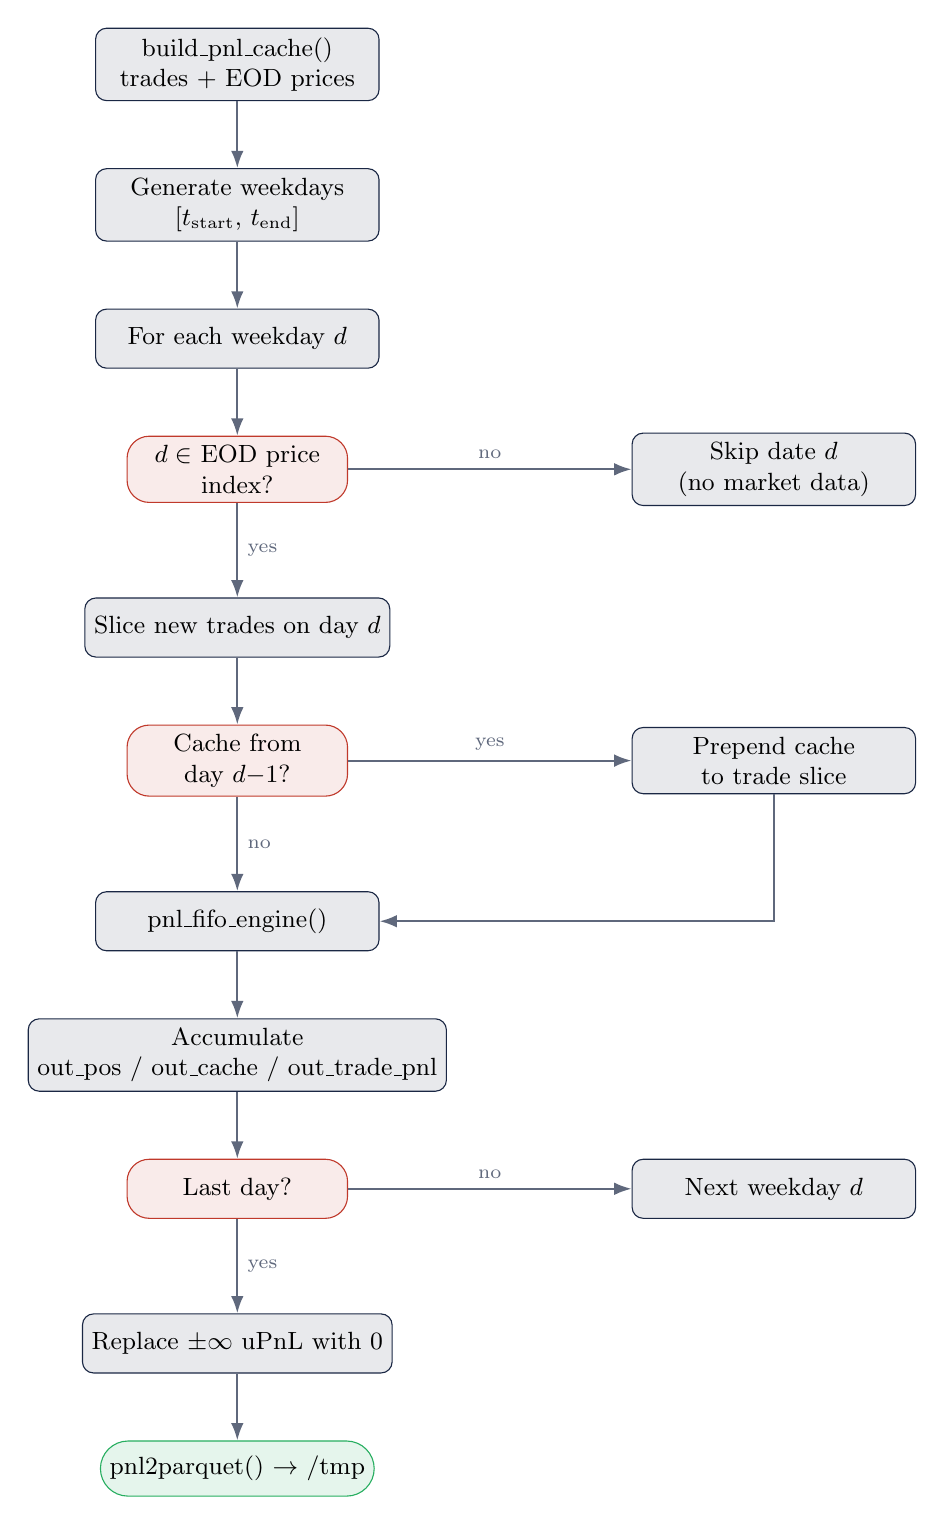
\begin{tikzpicture}[node distance=0.85cm and 0.5cm]

  \node[proc] (bc)
    {build\_pnl\_cache()\\trades + EOD prices};

  \node[proc, below=of bc] (wk)
    {Generate weekdays\\$[t_{\text{start}},\, t_{\text{end}}]$};

  \node[proc, below=of wk] (iter)
    {For each weekday $d$};

  \node[decide, below=of iter] (prx)
    {$d \in$ EOD price\\index?};

  \node[proc, right=3.6cm of prx] (skip2)
    {Skip date $d$\\(no market data)};

  \node[proc, below=1.2cm of prx] (tslice)
    {Slice new trades on day $d$};

  \node[decide, below=of tslice] (cache)
    {Cache from\\day $d{-}1$?};

  \node[proc, right=3.6cm of cache] (prepend)
    {Prepend cache\\to trade slice};

  \node[proc, below=1.2cm of cache] (eng)
    {pnl\_fifo\_engine()};

  \node[proc, below=of eng] (acc)
    {Accumulate\\out\_pos / out\_cache / out\_trade\_pnl};

  \node[decide, below=of acc] (last)
    {Last day?};

  \node[proc, right=3.6cm of last] (nxtd)
    {Next weekday $d$};

  \node[proc, below=1.2cm of last] (clean)
    {Replace $\pm\infty$ uPnL with 0};

  \node[cloud, below=of clean] (save)
    {pnl2parquet() $\to$ /tmp};

  \draw[arr] (bc)     -- (wk);
  \draw[arr] (wk)     -- (iter);
  \draw[arr] (iter)   -- (prx);
  \draw[arr] (prx)    -- node[above]{\scriptsize no}  (skip2);
  \draw[arr] (prx)    -- node[right]{\scriptsize yes} (tslice);
  \draw[arr] (tslice) -- (cache);
  \draw[arr] (cache)  -- node[above]{\scriptsize yes} (prepend);
  \draw[arr] (cache)  -- node[right]{\scriptsize no}  (eng);
  \draw[arr] (prepend) |- (eng);
  \draw[arr] (eng)    -- (acc);
  \draw[arr] (acc)    -- (last);
  \draw[arr] (last)   -- node[above]{\scriptsize no}  (nxtd);
  \draw[arr] (last)   -- node[right]{\scriptsize yes} (clean);
  \draw[arr] (clean)  -- (save);

\end{tikzpicture}
\caption{Day-by-day loop inside \texttt{initiate\_pnl\_engine}}
\end{figure}

\subsection{Cache Carry-Forward}

The FIFO queue must survive day boundaries.
At the end of day $d$ the \texttt{out\_cache} (residual open lots)
is prepended to the next day's trade slice before calling the engine:

\begin{equation}
  \mathcal{T}^{(d)} = \texttt{cache}^{(d-1)} \;\oplus\; \texttt{new\_trades}^{(d)}
\end{equation}

where $\oplus$ denotes chronologically-sorted row concatenation.
On day $d=0$ all trades from $t_{\text{start}}$ are loaded at once.

\subsection{Outputs}

\begin{tabular}{@{}lll@{}}
  \toprule
  Key                   & Type      & Content \\
  \midrule
  \texttt{out\_pos}        & DataFrame & Daily positions, rPnL, uPnL per symbol \\
  \texttt{out\_cache}      & DataFrame & Open FIFO lots to carry into next run \\
  \texttt{out\_trade\_pnl} & DataFrame & Trade-level realised P\&L \\
  \texttt{fname\_pnl}      & str       & Local path to position parquet \\
  \texttt{fname\_cache}    & str       & Local path to cache parquet \\
  \bottomrule
\end{tabular}

%% =============================================================
\section{\texttt{pnl\_realised\_polars} — FIFO Calculation Engine}

\subsection{Role in the Call Stack}

Inside \texttt{pnl\_fifo\_engine} the trade universe for each day is
split into two groups before P\&L is computed:

\begin{itemize}[noitemsep]
  \item \textbf{Non-CA symbols} (the majority) $\to$
        \texttt{pnl\_realised\_polars}
        \hfill \emph{(Polars-accelerated)}
  \item \textbf{Corporate-action symbols} $\to$
        \texttt{pnl\_realised\_ca}
        \hfill \emph{(handles split adjustments)}
\end{itemize}

\subsection{Input / Output}

\begin{tabular}{@{}lll@{}}
  \toprule
  Direction & Variable        & Description \\
  \midrule
  Input  & \texttt{df\_trades}   & pandas DataFrame with columns:
                                   \texttt{symbol, time, price, quantity, side} \\
  Output & \texttt{out\_pnl}     & Trade-level rPnL: \texttt{time, symbol, pnl, matched\_quantity} \\
  Output & \texttt{out\_cache}   & Residual open lots formatted for next-day carry-forward \\
  Output & \texttt{out\_pos}     & Position tracker: \texttt{time, symbol, trade\_price,}
                                   \texttt{trade\_quantity, short\_position} \\
  \bottomrule
\end{tabular}

\subsection{Internal Flow}

\begin{figure}[H]
\centering
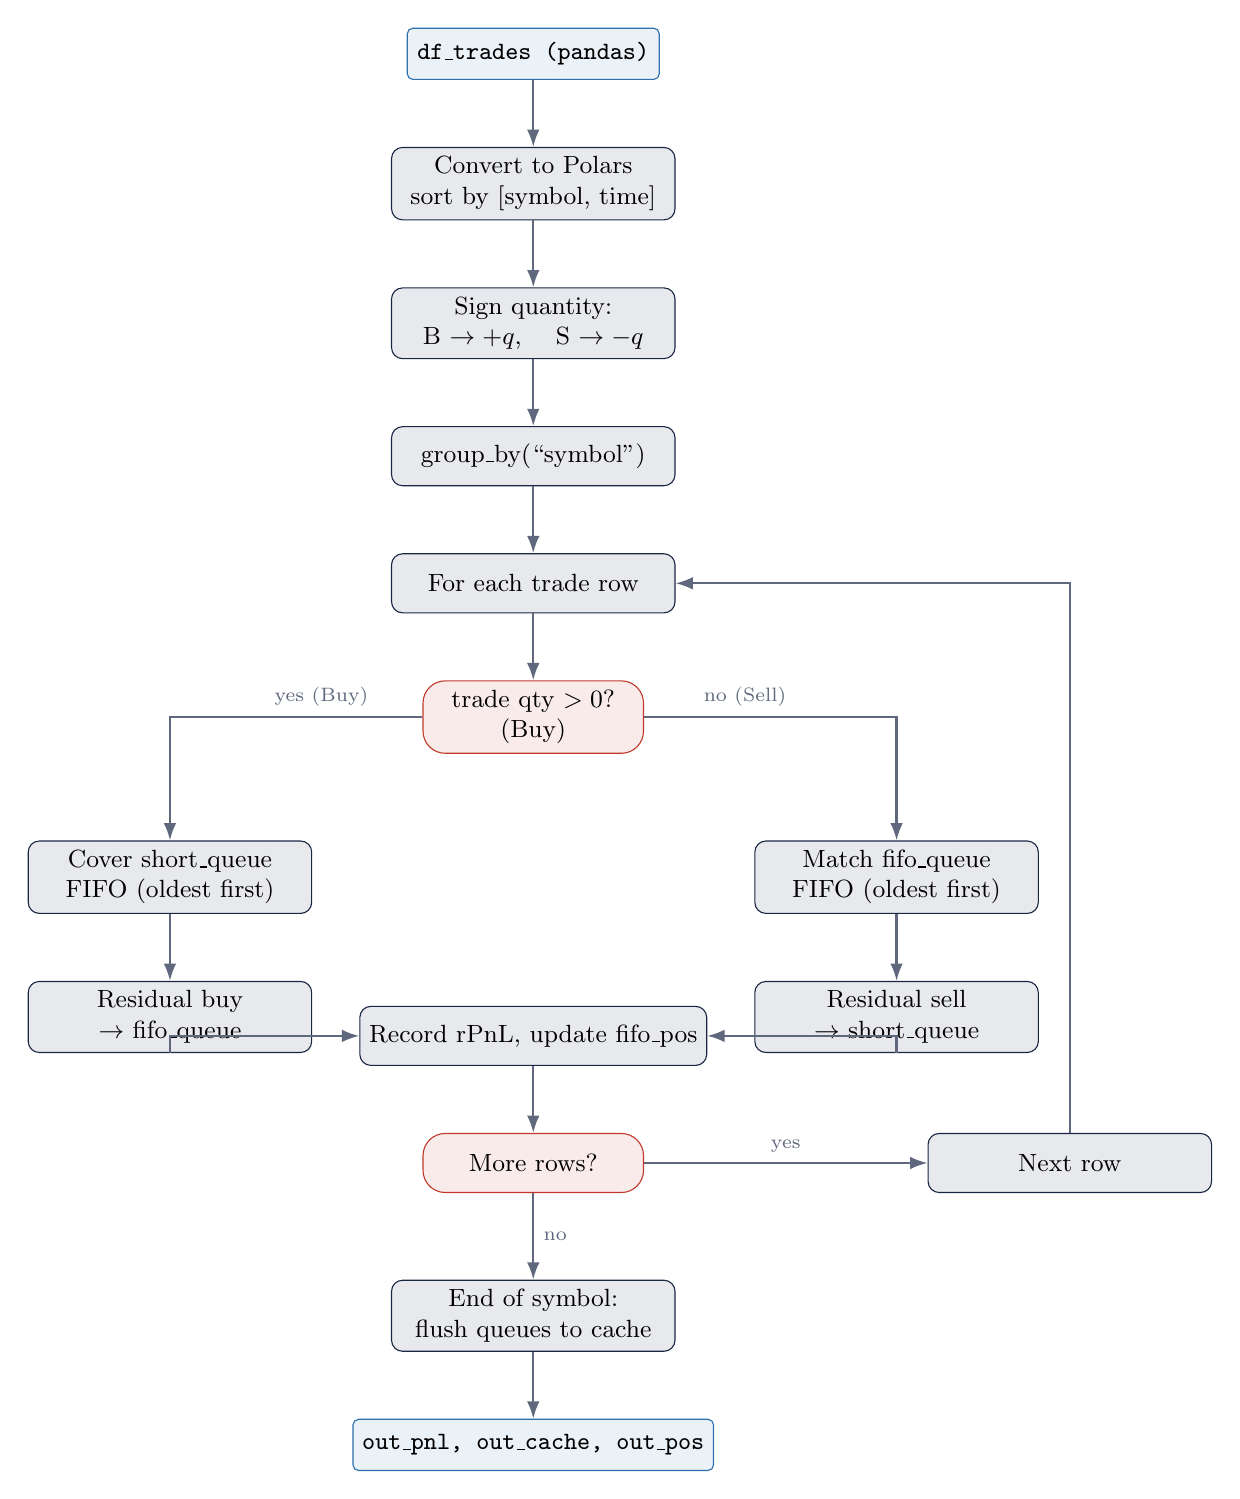
\begin{tikzpicture}[node distance=0.85cm and 0.5cm]

  \node[data] (inp)   {df\_trades (pandas)};

  \node[proc, below=of inp] (conv)
    {Convert to Polars\\sort by [symbol, time]};

  \node[proc, below=of conv] (sign)
    {Sign quantity:\\B $\to +q$, \quad S $\to -q$};

  \node[proc, below=of sign] (grp)
    {group\_by(``symbol'')};

  \node[proc, below=of grp] (row)
    {For each trade row};

  \node[decide, below=of row] (dir)
    {trade qty $> 0$?\\(Buy)};

  % Buy branch – LEFT
  \node[proc, below left=1.1cm and 1.4cm of dir] (cov)
    {Cover short\_queue\\FIFO (oldest first)};

  \node[proc, below=of cov] (enq)
    {Residual buy\\$\to$ fifo\_queue};

  % Sell branch – RIGHT
  \node[proc, below right=1.1cm and 1.4cm of dir] (mat)
    {Match fifo\_queue\\FIFO (oldest first)};

  \node[proc, below=of mat] (shq)
    {Residual sell\\$\to$ short\_queue};

  \node[proc, below=3.2cm of dir] (rec)
    {Record rPnL, update fifo\_pos};

  \node[decide, below=of rec] (eog)
    {More rows?};

  \node[proc, right=3.6cm of eog] (nextr)
    {Next row};

  \node[proc, below=1.1cm of eog] (flush)
    {End of symbol:\\flush queues to cache};

  \node[data, below=of flush] (out)
    {out\_pnl, out\_cache, out\_pos};

  \draw[arr] (inp)  -- (conv);
  \draw[arr] (conv) -- (sign);
  \draw[arr] (sign) -- (grp);
  \draw[arr] (grp)  -- (row);
  \draw[arr] (row)  -- (dir);
  \draw[arr] (dir)  -| node[above,pos=0.2]{\scriptsize yes (Buy)} (cov);
  \draw[arr] (dir)  -| node[above,pos=0.2]{\scriptsize no (Sell)} (mat);
  \draw[arr] (cov)  -- (enq);
  \draw[arr] (mat)  -- (shq);
  \draw[arr] (enq)  |- (rec);
  \draw[arr] (shq)  |- (rec);
  \draw[arr] (rec)  -- (eog);
  \draw[arr] (eog)  -- node[above]{\scriptsize yes} (nextr);
  \draw[arr] (nextr) |- (row);
  \draw[arr] (eog)  -- node[right]{\scriptsize no}  (flush);
  \draw[arr] (flush) -- (out);

\end{tikzpicture}
\caption{Internal control flow of \texttt{pnl\_realised\_polars}}
\end{figure}

\subsection{Data Structures}

Three queues are maintained \emph{per symbol}:

\begin{center}
\begin{tabular}{@{}llll@{}}
  \toprule
  Queue               & Entries            & Ordering   & Purpose \\
  \midrule
  \texttt{fifo\_queue}  & Unmatched buy lots & FIFO       & Match against future sells \\
  \texttt{short\_queue} & Unmatched sell lots & FIFO      & Match against future buys \\
  \texttt{fifo\_pnl}   & P\&L records       & Append-only & Collect rPnL per trade \\
  \bottomrule
\end{tabular}
\end{center}

\subsection{Mathematical Formulation}

\subsubsection{Sign Convention}

Let trade $i$ for symbol $s$ have timestamp $t_i$, execution price
$p_i$, and signed quantity

\begin{equation}
  q_i =
  \begin{cases}
    +\lvert q_i \rvert & \text{if } \texttt{side} = \texttt{B}
    \quad\text{(buy)} \\[4pt]
    -\lvert q_i \rvert & \text{if } \texttt{side} = \texttt{S}
    \quad\text{(sell)}
  \end{cases}
\end{equation}

\subsubsection{Sell Trade ($q_i < 0$): Long Book Realisation}

A sell is first matched against the \textbf{oldest} buy lots in
\texttt{fifo\_queue}.
Let lot $k$ carry price $p_k^{B}$ and remaining quantity $q_k^{B} > 0$.

\begin{align}
  m_{ik} &= \min\!\bigl(\lvert q_i^{\text{rem}}\rvert,\; q_k^{B}\bigr)
  \tag{matched quantity}\\[4pt]
  \text{rPnL}_{ik} &= m_{ik}\cdot\bigl(p_i - p_k^{B}\bigr)
  \label{eq:rpnl_sell}
  \tag{realised P\&L on sell}
\end{align}

After consuming the FIFO queue, any unmatched sell quantity is pushed
to \texttt{short\_queue} at price $p_i$:

\begin{equation}
  q_i^{\text{short}} = \lvert q_i \rvert - \sum_k m_{ik}
  \quad\text{(if } {>}\,0\text{)}
\end{equation}

\subsubsection{Buy Trade ($q_i > 0$): Short Cover}

A buy first covers open short lots in \texttt{short\_queue}.
Let lot $j$ carry price $p_j^{S}$ and remaining quantity $q_j^{S} > 0$.

\begin{align}
  m_{ij} &= \min\!\bigl(q_i^{\text{rem}},\; q_j^{S}\bigr)
  \tag{matched quantity}\\[4pt]
  \text{rPnL}_{ij} &= m_{ij}\cdot\bigl(p_j^{S} - p_i\bigr)
  \label{eq:rpnl_buy}
  \tag{realised P\&L on short cover}
\end{align}

After covering shorts, any unmatched buy quantity joins the FIFO queue:

\begin{equation}
  q_i^{\text{FIFO}} = q_i - \sum_j m_{ij}
  \quad\text{(if } {>}\,0\text{)}
\end{equation}

\subsubsection{Total Realised P\&L per Trade}

\begin{equation}
  \boxed{%
    \text{rPnL}_i
    = \underbrace{\sum_j m_{ij}\cdot(p_j^S - p_i)}_{\text{short cover gain}}
    + \underbrace{\sum_k m_{ik}\cdot(p_i - p_k^B)}_{\text{long book gain}}
  }
\end{equation}

For a pure long-only book (no shorts), only the second term is
non-zero.

\subsubsection{Unrealised P\&L}

After the FIFO loop the residual open lots from both queues
constitute the \emph{end-of-day open position}.
Using the EOD market price $P_t^{\text{EOD}}$:

\begin{equation}
  \text{uPnL}_\ell^{(t)} =
    \bigl(P_t^{\text{EOD}} - p_\ell\bigr)\cdot q_\ell^{\text{open}}
  \label{eq:upnl}
\end{equation}

Aggregating over all open lots for symbol $s$:

\begin{equation}
  \text{uPnL}_s^{(t)} =
    \sum_{\ell \in \text{open}(s)}
    \bigl(P_t^{\text{EOD}} - p_\ell\bigr)\cdot q_\ell^{\text{open}}
\end{equation}

\subsubsection{P\&L Identity}

Over a horizon $[t_0, T]$ the total P\&L satisfies:

\begin{equation}
  \text{Total PnL}^{(T)} =
    \underbrace{\sum_i \text{rPnL}_i}_{\text{cumulative realised}}
    +\underbrace{\text{uPnL}^{(T)}}_{\text{mark-to-market}}
\end{equation}

This identity holds by construction: every traded unit either
generated a realised P\&L at the moment of matching, or remains
as an open lot valued at the current market price.

%% =============================================================
\section{FIFO Matching Examples}

\subsection{Standard Sell Against Long Book}

\begin{figure}[H]
\centering
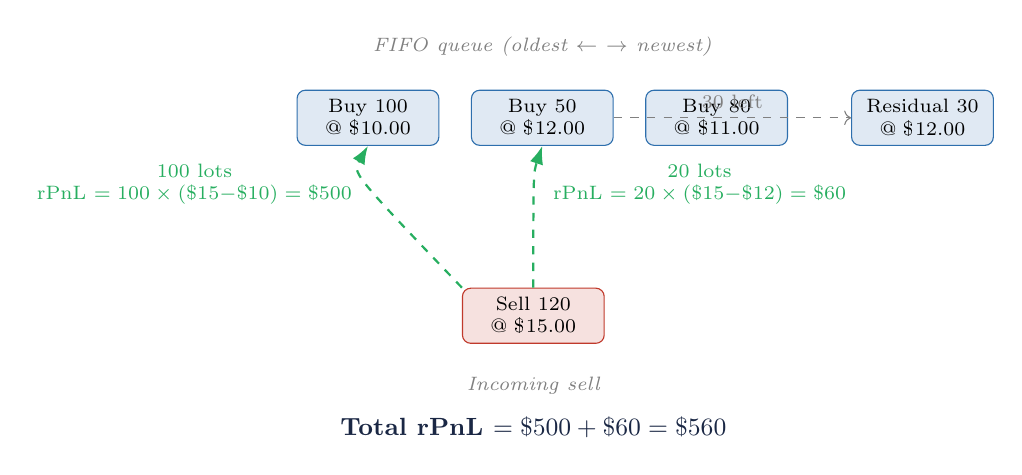
\begin{tikzpicture}[node distance=1.0cm and 0.3cm]

  \node[lot] (b1) {Buy 100\\@ \$10.00};
  \node[lot, right=0.4cm of b1] (b2) {Buy 50\\@ \$12.00};
  \node[lot, right=0.4cm of b2] (b3) {Buy 80\\@ \$11.00};

  \node[font=\scriptsize\itshape, color=gray, above=0.3cm of b2]
    {FIFO queue (oldest $\leftarrow$ $\rightarrow$ newest)};

  \node[sell, below=1.8cm of b1, xshift=2.1cm] (s1)
    {Sell 120\\@ \$15.00};

  \node[font=\scriptsize\itshape, color=gray, below=0.3cm of s1]
    {Incoming sell};

  \draw[-{Latex}, dashed, TR_GREEN, thick]
    (s1.north west) .. controls (-0.2, -0.7) .. (b1.south)
    node[midway, left=2pt, font=\scriptsize, color=TR_GREEN, align=center]
    {100 lots\\rPnL $= 100\times(\$15{-}\$10) = \$500$};

  \draw[-{Latex}, dashed, TR_GREEN, thick]
    (s1.north) .. controls (2.1,-0.7) .. (b2.south)
    node[midway, right=3pt, font=\scriptsize, color=TR_GREEN, align=center]
    {20 lots\\rPnL $= 20\times(\$15{-}\$12) = \$60$};

  \node[lot, right=0.8cm of b3] (b2r) {Residual 30\\@ \$12.00};
  \draw[->, dashed, gray] (b2.east)
    -- node[above]{\scriptsize 30 left} (b2r.west);

  \node[font=\small\bfseries, color=TR_DARK, below=0.8cm of s1]
    {Total rPnL $= \$500 + \$60 = \$560$};

\end{tikzpicture}
\caption{Sell 120 lots matched against two FIFO buy lots}
\end{figure}

\subsection{Sell Exceeds Available Longs — Short Queue Created}

\begin{figure}[H]
\centering
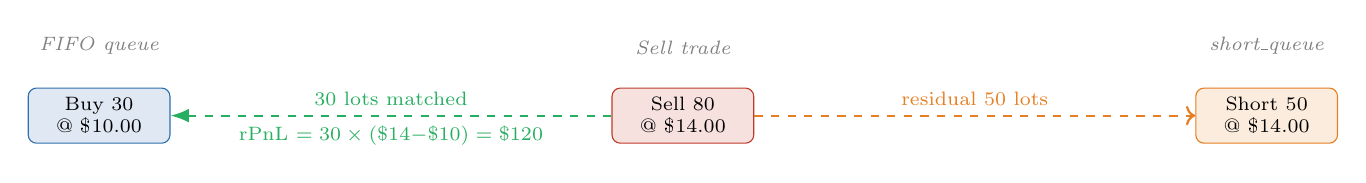
\begin{tikzpicture}[node distance=1.4cm and 0.4cm]

  \node[lot] (b1) {Buy 30\\@ \$10.00};
  \node[font=\scriptsize\itshape, color=gray, above=0.3cm of b1]
    {FIFO queue};

  \node[sell, right=5.6cm of b1] (s1) {Sell 80\\@ \$14.00};
  \node[font=\scriptsize\itshape, color=gray, above=0.3cm of s1]
    {Sell trade};

  \draw[-{Latex}, dashed, TR_GREEN, thick]
    (s1.west) --
    node[above, font=\scriptsize, align=center]{30 lots matched}
    node[below, font=\scriptsize, color=TR_GREEN, align=center]
      {rPnL $= 30\times(\$14{-}\$10) = \$120$}
    (b1.east);

  \node[shq, right=5.6cm of s1] (sq)
    {Short 50\\@ \$14.00};
  \node[font=\scriptsize\itshape, color=gray, above=0.3cm of sq]
    {short\_queue};
  \draw[->, dashed, TR_ORANGE, thick]
    (s1.east) -- node[above, font=\scriptsize]{residual 50 lots} (sq.west);

\end{tikzpicture}
\caption{Short queue created when sell quantity exceeds available FIFO lots}
\end{figure}

%% =============================================================
\section{Key Implementation Notes}

\begin{enumerate}

  \item \textbf{Polars for I/O, Python loop for matching.}
    The input DataFrame is converted to Polars once and sorted via
    the Polars engine (fast columnar sort).  The per-row FIFO
    matching loop itself is a plain Python \texttt{for} loop —
    correctness is prioritised over vectorisation for the stateful
    queue logic.

  \item \textbf{Short-price preservation.}
    Each short lot in \texttt{short\_queue} retains its
    \emph{individual} execution price rather than being
    averaged.  This avoids P\&L mis-attribution when multiple
    short trades are opened at different prices and later covered
    individually.

  \item \textbf{Corporate-action isolation.}
    Symbols with \texttt{booking\_category == 'CORPORATE\_ACTION'}
    are routed to \texttt{pnl\_realised\_ca}, which adjusts
    historical quantities by the split ratio before applying FIFO.

  \item \textbf{Missing price handling.}
    Trades with a null price in the source are backfilled from the
    EOD price series inside \texttt{build\_pnl\_cache}; any
    still-null prices are set to 1 to prevent silent row drops.

  \item \textbf{Excluded ISINs.}
    Three ISINs are hard-coded out of the trade feed due to known
    data quality issues:\\
    \texttt{US33817P3064}, \texttt{NL0012047823}, \texttt{US03815U6073}.

  \item \textbf{uPnL edge-case cleanup.}
    After the day loop, \texttt{initiate\_pnl\_engine} replaces
    $\pm\infty$ values in the uPnL column with 0; these can arise
    when the EOD price for an open lot is missing.

\end{enumerate}

%% =============================================================
\section{Infrastructure: AWS ECR \& Airflow Orchestration}

\subsection{Docker Image on AWS ECR}

The entire \texttt{risk\_pylibrary} codebase is containerised and
pushed to AWS Elastic Container Registry (ECR) on every merge to
\texttt{main}:

\begin{mdframed}[backgroundcolor=TR_GRAY, linecolor=TR_BLUE,
                 linewidth=1pt, roundcorner=4pt]
\texttt{263932266204.dkr.ecr.eu-central-1.amazonaws.com/risk/risk\_pylibrary:\textbf{main}}
\end{mdframed}

\medskip
The container entrypoint used by the Airflow task is:

\begin{lstlisting}[style=pycode]
python /usr/local/app/automation/task_pnl_trading_book.py
\end{lstlisting}

Resource allocation on AWS Fargate:

\begin{center}
\begin{tabular}{@{}lll@{}}
  \toprule
  Resource & Request & Limit \\
  \midrule
  Memory & 16\,GiB & 16\,GiB \\
  CPU    & 4\,000\,m (4 vCPU) & 4\,000\,m \\
  \bottomrule
\end{tabular}
\end{center}

The 16\,GiB allocation is driven by the in-memory FIFO queue for
all four accounts across a multi-month trade history loaded at
once during the cache build step.

\subsection{Snowflake Credentials Injection}

Snowflake credentials are never baked into the image.
They are injected at runtime via Kubernetes Secrets from the
service account \texttt{airflow-risk-service-function-credentials},
mapped to the following environment variables inside the container:

\begin{center}
\begin{tabular}{@{}ll@{}}
  \toprule
  Environment Variable      & Secret Key \\
  \midrule
  \texttt{SNOWFLAKE\_ACCOUNT}   & \texttt{dbt-snowflake-account-id} \\
  \texttt{SNOWFLAKE\_USERNAME}  & \texttt{dbt-snowflake-user} \\
  \texttt{SNOWFLAKE\_PASSWORD}  & \texttt{dbt-snowflake-password} \\
  \texttt{SNOWFLAKE\_ROLE}      & \texttt{dbt-snowflake-role} \\
  \texttt{SNOWFLAKE\_DATABASE}  & \texttt{dbt-snowflake-database} \\
  \texttt{SNOWFLAKE\_WAREHOUSE} & \texttt{dbt-snowflake-warehouse} \\
  \bottomrule
\end{tabular}
\end{center}

The pod runs under the Kubernetes service account
\texttt{risk-function-models-airflow}, which carries the IAM role
binding for S3 write access to \texttt{tr-risk-data-prd}.

\subsection{Airflow DAG}

\begin{mdframed}[backgroundcolor=TR_GRAY, linecolor=TR_BLUE,
                 linewidth=1pt, roundcorner=4pt]
\textbf{DAG ID:}
  \texttt{risk\_function.risk\_function\_mrm\_trading\_eod\_pnl}\\[4pt]
\textbf{Schedule:} \texttt{None} (triggered externally or manually)\\[4pt]
\textbf{Owner:} \texttt{Element.COMPLIANCE\_AND\_RISK}\\[4pt]
\textbf{Tags:}
  \texttt{risk\_function}, \texttt{risk\_function\_mrm},
  \texttt{mrm\_ecr}, \texttt{trading\_book\_pnl}
\end{mdframed}

\subsubsection{DAG Workflow}

\begin{figure}[H]
\centering
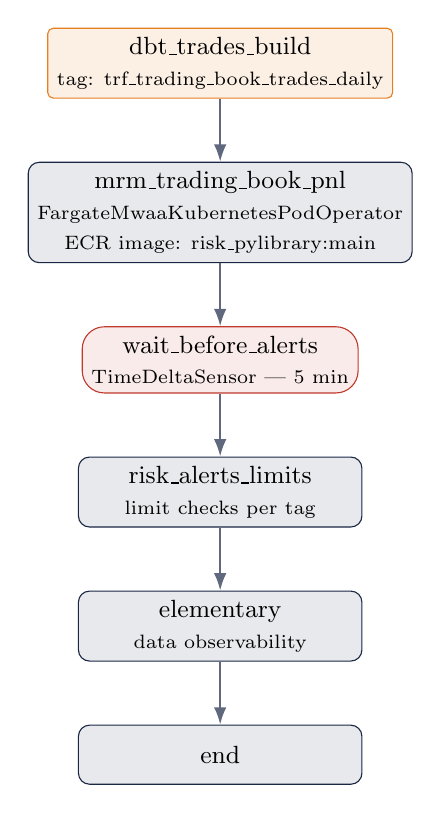
\begin{tikzpicture}[node distance=0.8cm and 0.3cm]

  \node[dbbox] (dbt)
    {dbt\_trades\_build\\{\scriptsize tag: trf\_trading\_book\_trades\_daily}};

  \node[proc, below=of dbt] (ecr)
    {mrm\_trading\_book\_pnl\\{\scriptsize FargateMwaaKubernetesPodOperator}\\{\scriptsize ECR image: risk\_pylibrary:main}};

  \node[decide, below=of ecr] (wait)
    {wait\_before\_alerts\\{\scriptsize TimeDeltaSensor — 5 min}};

  \node[proc, below=of wait] (alerts)
    {risk\_alerts\_limits\\{\scriptsize limit checks per tag}};

  \node[proc, below=of alerts] (elem)
    {elementary\\{\scriptsize data observability}};

  \node[proc, below=of elem] (end) {end};

  \draw[arr] (dbt)    -- (ecr);
  \draw[arr] (ecr)    -- (wait);
  \draw[arr] (wait)   -- (alerts);
  \draw[arr] (alerts) -- (elem);
  \draw[arr] (elem)   -- (end);

\end{tikzpicture}
\caption{Airflow DAG task sequence for
  \texttt{risk\_function\_mrm\_trading\_eod\_pnl}}
\end{figure}

\subsubsection{Task Descriptions}

\begin{enumerate}[noitemsep]

  \item \textbf{\texttt{dbt\_trades\_build}} —
        Runs \texttt{dbt build --select tag:trf\_trading\_book\_trades\_daily}
        via \texttt{DbtKubernetesPodOperator}.
        This materialises the cleaned daily trade source tables in
        Snowflake that \texttt{task\_pnl\_trading\_book.py} reads.

  \item \textbf{\texttt{mrm\_trading\_book\_pnl}} —
        Pulls the ECR image and executes
        \texttt{task\_pnl\_trading\_book.py} on AWS Fargate
        (16\,GiB / 4\,vCPU).
        Startup timeout is 500\,s.
        The pod is \emph{not} deleted on completion
        (\texttt{is\_delete\_operator\_pod=False}) to allow log
        inspection after the run.

  \item \textbf{\texttt{wait\_before\_alerts}} —
        A \texttt{TimeDeltaSensor} that holds the pipeline for
        5\,minutes after the PnL task finishes.
        This gives downstream Snowflake materialisation time to
        complete before limit checks are evaluated.

  \item \textbf{\texttt{risk\_alerts\_limits}} —
        Runs limit-breach checks against the freshly written PnL
        data, filtered by tag \texttt{risk\_function\_mrm\_trading\_eod\_pnl}.
        Generates alerts if any configured thresholds are breached.

  \item \textbf{\texttt{elementary}} —
        Triggers the Elementary data-observability suite on
        \texttt{tags:risk\_function\_mrm\_model\_pnl} to validate
        data quality (row counts, freshness, schema drift).

\end{enumerate}

%% =============================================================
\section{Full Call-Stack Summary}

\begin{figure}[H]
\centering
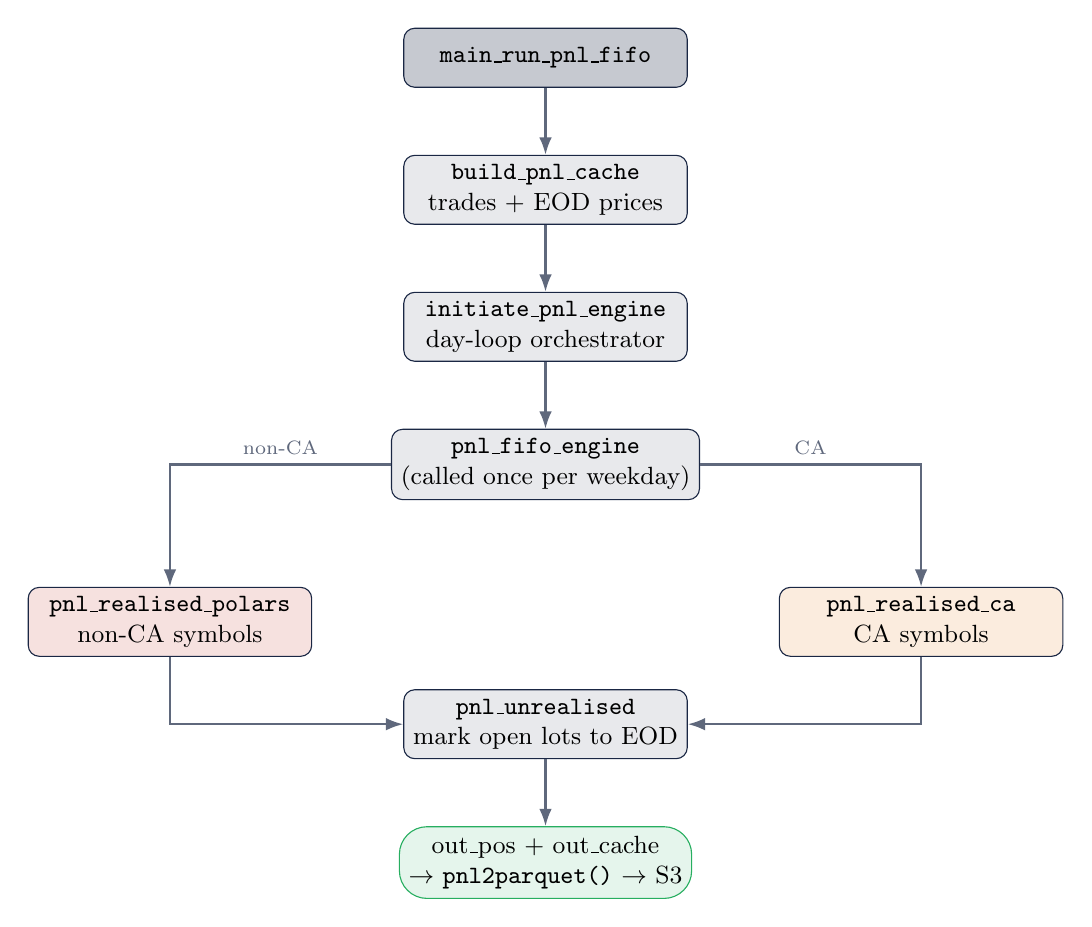
\begin{tikzpicture}[node distance=0.85cm and 0.2cm]

  \node[proc, fill=TR_DARK!25] (t1)
    {\texttt{main\_run\_pnl\_fifo}};

  \node[proc, below=of t1] (t2)
    {\texttt{build\_pnl\_cache}\\trades + EOD prices};

  \node[proc, below=of t2] (t3)
    {\texttt{initiate\_pnl\_engine}\\day-loop orchestrator};

  \node[proc, below=of t3] (t4)
    {\texttt{pnl\_fifo\_engine}\\(called once per weekday)};

  \node[proc, below left=1.1cm and 1.0cm of t4, fill=TR_RED!15] (t5a)
    {\texttt{pnl\_realised\_polars}\\non-CA symbols};

  \node[proc, below right=1.1cm and 1.0cm of t4, fill=TR_ORANGE!15] (t5b)
    {\texttt{pnl\_realised\_ca}\\CA symbols};

  \node[proc, below=2.4cm of t4] (t6)
    {\texttt{pnl\_unrealised}\\mark open lots to EOD};

  \node[cloud, below=of t6] (out)
    {out\_pos + out\_cache\\$\to$ \texttt{pnl2parquet()} $\to$ S3};

  \draw[arr] (t1) -- (t2);
  \draw[arr] (t2) -- (t3);
  \draw[arr] (t3) -- (t4);
  \draw[arr] (t4) -| node[above,pos=0.25]{\scriptsize non-CA} (t5a);
  \draw[arr] (t4) -| node[above,pos=0.25]{\scriptsize CA}     (t5b);
  \draw[arr] (t5a) |- (t6);
  \draw[arr] (t5b) |- (t6);
  \draw[arr] (t6)  -- (out);

\end{tikzpicture}
\caption{Complete call stack from Airflow task to S3 output}
\end{figure}

%% =============================================================
\appendix
\section{Source Code: \texttt{pnl\_realised\_polars}}
\label{app:code}

Full source of \texttt{risk\_models/pnl\_fifo.py} —
function \texttt{pnl\_realised\_polars} (lines 577\,--\,728).

\begin{lstlisting}[style=pycode, numbers=left, firstnumber=577,
  xleftmargin=2em, framexleftmargin=2em]
def pnl_realised_polars(df_trades):
    """
    Calculate FIFO PnL using polars, ensuring that each residual short trade
    retains its specific price instead of averaging.

    Parameters:
        df_trades (pd.DataFrame): Input data with columns:
            - 'symbol': Asset identifier.
            - 'time': Trade date.
            - 'price': Trade execution price.
            - 'quantity': Positive for buys, negative for sells.

    Returns:
        tuple: Three DataFrames containing:
            - PnL results per trade
            - Remaining FIFO queue
            - Position tracking
    """
    # Convert to Polars DataFrame and sort by symbol and date
    df = pl.from_pandas(df_trades).sort(by=["symbol", "time"])

    # Mapping positive and negative signs for trade direction
    df = df.with_columns(
        pl.when(pl.col("side") == "B")
          .then(pl.col("quantity"))
          .otherwise(-1 * pl.col("quantity"))
          .alias("quantity")
    )

    # Group by symbol and process each group
    results = []
    cache   = []
    pos     = []

    for group in df.group_by("symbol"):
        trades_orig = group[1]
        trades = trades_orig.filter(pl.col("price").is_not_null())

        # Per-symbol queues
        fifo_queue  = []   # unmatched buy lots {time, symbol, quantity, price}
        fifo_pnl    = []   # realised PnL records
        fifo_pos    = []   # position tracker
        short_queue = []   # individual short lots (price preserved, not averaged)

        for row in trades.iter_rows(named=True):
            trade_quantity = row["quantity"]
            trade_price    = row["price"]
            realized_pnl   = 0.0
            match_quantity = 0.0

            # ----------------------------------------------------------
            # BUY trade: cover shorts first, then enqueue remainder
            # ----------------------------------------------------------
            if trade_quantity > 0:
                while trade_quantity > 0 and short_queue:
                    short_trade    = short_queue[0]
                    match_quantity = min(trade_quantity, short_trade["quantity"])
                    # Short cover: gain = (short price - buy price) * matched qty
                    realized_pnl  += match_quantity * (short_trade["price"] - trade_price)

                    short_trade["quantity"] -= match_quantity
                    trade_quantity          -= match_quantity

                    if short_trade["quantity"] == 0:
                        short_queue.pop(0)

                fifo_pos.append({
                    "time":           row["time"],
                    "symbol":         row["symbol"],
                    "trade_price":    trade_price,
                    "trade_quantity": trade_quantity,
                    "short_position": sum(t["quantity"] for t in short_queue),
                    "match_quantity": match_quantity,
                })

                # Remaining buy quantity -> FIFO queue
                if trade_quantity > 0:
                    fifo_queue.append({
                        "time":     row["time"],
                        "symbol":   row["symbol"],
                        "quantity": trade_quantity,
                        "price":    trade_price,
                    })

            # ----------------------------------------------------------
            # SELL trade: match against FIFO queue, overflow -> short queue
            # ----------------------------------------------------------
            elif trade_quantity < 0:
                sell_quantity = -trade_quantity

                while sell_quantity > 0 and fifo_queue:
                    buy_trade      = fifo_queue[0]
                    match_quantity = min(sell_quantity, buy_trade["quantity"])
                    # Long realisation: gain = (sell price - buy price) * matched qty
                    realized_pnl  += match_quantity * (trade_price - buy_trade["price"])

                    buy_trade["quantity"] -= match_quantity
                    sell_quantity         -= match_quantity

                    if buy_trade["quantity"] == 0:
                        fifo_queue.pop(0)

                # Unmatched sell residual stored with its own price (not averaged)
                if sell_quantity > 0:
                    short_queue.append({
                        "time":     row["time"],
                        "symbol":   row["symbol"],
                        "quantity": sell_quantity,
                        "price":    trade_price,
                    })

                fifo_pos.append({
                    "time":           row["time"],
                    "symbol":         row["symbol"],
                    "trade_price":    trade_price,
                    "trade_quantity": trade_quantity,
                    "short_position": sum(t["quantity"] for t in short_queue),
                    "match_quantity": match_quantity,
                })

            # Record PnL for this trade (0.0 if no match occurred)
            fifo_pnl.append({
                "time":             row["time"],
                "symbol":           row["symbol"],
                "pnl":              realized_pnl,
                "matched_quantity": match_quantity,
            })

        # Flush short_queue into cache with negated quantities (sign convention)
        if len(short_queue) > 0:
            short_queue = [{**p, "quantity": -1 * p["quantity"]} for p in short_queue]

        cache.extend(short_queue)
        results.extend(fifo_pnl)
        cache.extend(fifo_queue)
        pos.extend(fifo_pos)

    # Convert results back to pandas
    out_pnl   = pd.DataFrame(results)
    out_cache = pd.DataFrame(cache)
    out_pos   = pd.DataFrame(pos)

    # Format cache for next-day carry-forward
    out_cache["side"]             = np.where(out_cache["quantity"] < 0, "S", "B")
    out_cache["booking_type"]     = np.where(out_cache["quantity"] < 0, "SELL", "BUY")
    out_cache["quantity"]         = out_cache["quantity"].abs()
    out_cache["booking_category"] = "TRADING"
    out_cache["multiplier"]       = 1
    out_cache = out_cache[[
        "time", "symbol", "side", "booking_category",
        "booking_type", "price", "quantity", "multiplier",
    ]]

    return out_pnl, out_cache, out_pos
\end{lstlisting}

\end{document}
